\documentclass{beamer}
\usepackage[utf8]{inputenc}
\usepackage{tikz}
\usepackage{verbatim}
\usetheme{Darmstadt}
\title{Introduction to CouchDB}
\author{Ondřej Kupka}

\AtBeginSection[]
{
  \begin{frame}<beamer>
    \frametitle{Section Layout}
    \tableofcontents[currentsection]
  \end{frame}
}

\begin{document}

\begin{frame}
\titlepage
\end{frame}

\section{The Big Picture}
\subsection{Current Situation}
\begin{frame}{Current Situation on the Databases Market}
  \begin{itemize}
    \item RDBMS are de facto an industrial standard
    \begin{itemize}
      \item Solid theoretical background
      \item Implementations proven by time
      \item Commercial support provided by large companies
      \item Widespread
    \end{itemize}
    \item RDBMS do have something to offer
    \begin{itemize}
      \item Suitable for any data model that can be captured in relations
      \item Ad-hoc queries (run time flexibility)
      \item Consistency (transactions)
    \end{itemize}
  \end{itemize}
\end{frame}

\begin{frame}{New Challenges}
  With the advent of web-scale applications, we are facing many new~challenges.
  Huge amount of loosely structured data needs to~be processed.
  What we seek is:
  \begin{itemize}
    \item Good scalability while retaining consistency
    \item High performance
    \item High availability and robustness
  \end{itemize}
  We are, however, not living in a dreamworld \ldots
\end{frame}

\subsection{A Bit of Theory}
\begin{frame}{CAP (Brewer's) Theorem}
  No distributed computer system can simultaneously provide\\all of
  the following guarantees:
  \begin{itemize}
    \item Consistency
    \item Availability
    \item Partition tolerance
  \end{itemize}
  \begin{center}
    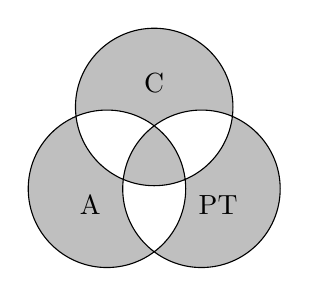
\begin{tikzpicture}
      \filldraw[fill=lightgray,even odd rule]
        (60:1.2) circle (1) ++(90:0.3) node{C}
        (0:0) circle (1) ++(225:0.3) node{A}
        (0:1.2) circle (1) ++(315:0.3) node{PT};
    \end{tikzpicture}
  \end{center}
  \fontsize{6}{8}\selectfont
  Began as a conjecture by Eric Brewer in 2000 and was proven by Seth Gilbert
  and Nancy Lynch of MIT in 2002.\\
\end{frame}

\begin{frame}{Consistency Model Revised}
  We could leverage our requirements a bit in a distributed environment,
  which would bring some issues, but also major befits.\\
  It looks like it is worth it :-)
  \begin{description}
    \item[ACID] (pesimistic - Consistency + Availability) \hfill
    \begin{enumerate}
      \item Atomicity
      \item Consistency
      \item Isolation
      \item Durability
    \end{enumerate}
    \item[BASE] (optimistic - Availability + Partition tolerance) \hfill
    \begin{enumerate}
      \item Basically Available
      \item Soft state
      \item Eventual consistency
    \end{enumerate}
  \end{description} 
\end{frame}

\subsection{The NoSQL Movement}
\begin{frame}{History and Core Principles}
  \begin{itemize}
    \item In 1998 Carlo Strozzi used the term to name light-weight DBs with no SQL,
          and also no relations. He then suggested to call them 'NoREL'.
    \item Reintroduced by Eric Evans of Rackspace in 2009 to name\\a growing
          number of non-relational distributed DBs\\not attemping to provide ACID.
    \item Today it is usually translated as 'Not only SQL'.
    \item In 2011, work began on UnQL, a query language for NoSQL databases.
          Does not cover the data definition.
  \end{itemize}
\end{frame}

\begin{frame}{Characteristics}
  Among the ideas characterizing NoSQL databases are:
  \begin{itemize}
    \item High optimisation for just the basic (CRUD) operations
    \item Providing little functionality beyond record storage
    \item Trading run time flexibility for gains in performance and scalability
          for certain data models (specialization)
    \item No SQL as the query language
    \item No ACID guarantees (BASE)
    \item Distributed and fault-tolerant
  \end{itemize}
  So basically we get systems that are hard to bring down and are able to handle
  enormous amount of data, but they are sacrificing functionality for that.
  If you, however, pick up the right system for you, it can do magic.
\end{frame}

\begin{frame}{Taxonomy of NoSQL Databases}
  \begin{itemize}
    \item Key-value stores
    \item \alert<2>{Document stores}
    \item Column families
    \item Graph databases
    \item Tuple/RDF stores
    \item XML databases
    \item Object stores
    \item \ldots
  \end{itemize}
\end{frame}

\begin{frame}[fragile]{Document Stores}
  \framesubtitle{What they are}
  You can imagine a document store as a key-value store,\\but the database begins
  to understand the structure of values (called 'documents') stored in there,
  which implies:
  \begin{itemize}
    \item Need for particular encoding of the data (XML, JSON, \ldots),
          but still no structure (no hard-coded schemas)
    \item It is possible to query the data (and do computations - MapReduce)
    \item It works in a CRUD way, a document being the basic unit.
          Operations on documents are usually the only atomic thing.
  \end{itemize}
  \fontsize{8}{10}\selectfont
  \begin{verbatim}
  { "firstName": "John", "lastName": "Smith" }
  \end{verbatim}
  Examples: MongoDB, \alert<2>{CouchDB}, RavenDB (transactions!)
\end{frame}

\begin{frame}{Document Stores}
  \framesubtitle{Limitations}
  \begin{itemize}
    \item They are not a general-purpose databases
    \begin{itemize}
      \item They require a special care while designing an application
    \end{itemize}
    \item Lack of run time flexibility, no relations you can join
    \item The basic units are documents, not fields inside of them
    \begin{itemize}
      \item Difficult to change a single piece of information if in many docs
    \end{itemize}
  \end{itemize}
\end{frame}

\section{CouchDB}
\subsection{Introduction}
\begin{frame}[fragile]{Before We Start}
  \framesubtitle{Installing and Starting CouchDB}
  Let us set up CouchDB so that we can try what we have learned immediately!
  Change defaults for production! There is a webmin called Futon
  bundled with CouchDB that you can use...
  \fontsize{6}{8}\selectfont
  \begin{verbatim}
  $ brew install couchdb # or apt-get install or whatever...
  $ couchdb
  Apache CouchDB 1.2.0 (LogLevel=info) is starting.
  Apache CouchDB has started. Time to relax.
  [info] [<0.31.0>] Apache CouchDB has started on http://127.0.0.1:5984/
  ...

  $ open http://127.0.0.1:5984/_utils # for Futon
  \end{verbatim}
\end{frame}

\begin{frame}{Overview and Core Features}
  \begin{itemize}
    \item Initial release in 2005, Apache project in 2008 (OSS)
    \item \textit{A database that completely embraces the web}
    \begin{itemize}
      \item Store JSON documents
      \item Access them via HTTP
      \item Query, combine and transform data with JavaScript
      \item Even serve applications directly out of CouchDB
    \end{itemize}
    \item ACID semantics (Multi-Version Concurrency Control)
    \item Eventual consistency
    \item Built for being offline (Partition tolerance)
    \item Distributed architecture with replication
    \item MapReduce views, and indexes
    \item REST API
  \end{itemize}
\end{frame}

\subsection{Document Storage}
\begin{frame}[fragile]{Basics}
  \begin{itemize}
    \item Server stores named databases, which contain\\JSON documents (mostly)
    \item Documents are primary units of data; they have any number of fields
          and attachments, and database metadata like id\\and revision
    \item Update model is optimistic and lockless
    \begin{itemize}
      \item load - modify - save not atomic, MVCC used to signal conflicts
    \end{itemize}
  \end{itemize}
  \fontsize{6}{8}\selectfont
  \begin{verbatim}
  {"_id":"89027e7860926e4815267048520017df","_rev":"1-bfb0d347cff4cb38161d90ea749fe2a0",
   "firstname":"Ondrej","surname":"Kupka"}
  \end{verbatim}
\end{frame}

\begin{frame}[fragile]{Demo 1}
  \framesubtitle{Database and Document Creation}
  \fontsize{6}{8}\selectfont
  \begin{verbatim}
  $ curl -X PUT http://127.0.0.1:5984/testdb
  {"ok":true}
  $ curl -X GET http://127.0.0.1:5984/_uuids
  {"uuids":["89027e7860926e4815267048520017ec"]}
  $ curl -X PUT http://127.0.0.1:5984/testdb/89027e7860926e4815267048520017ec \
  > -d '{"firstname":"Ondrej","surname":"Kupka"}'
  {"ok":true,"id":"89027e7860926e4815267048520017ec","rev":"1-bfb0d347cff4cb38161d90ea749fe2a0"}
  \end{verbatim}
\end{frame}

\begin{frame}[fragile]{Demo 2}
  \framesubtitle{Conflict Occurence and Resolution}
  \fontsize{6}{8}\selectfont
  \begin{verbatim}
  ME$ curl -X GET http://127.0.0.1:5984/testdb/89027e7860926e4815267048520017ec
  {"_id":"89027e7860926e4815267048520017ec","_rev":"1-bfb0d347cff4cb38161d90ea749fe2a0",
   "firstname":"Ondrej","surname":"Kupka"}

  HIM$ curl -X GET http://127.0.0.1:5984/testdb/89027e7860926e4815267048520017ec
  {"_id":"89027e7860926e4815267048520017ec","_rev":"1-bfb0d347cff4cb38161d90ea749fe2a0",
   "firstname":"Ondrej","surname":"Kupka"}

  HIM$ curl -X PUT http://127.0.0.1:5984/testdb/89027e7860926e4815267048520017ec \
  >  -d '{"_rev":"1-bfb0d347cff4cb38161d90ea749fe2a0","firstname":"Ondrej","surname":"Krupka"}'
  {"ok":true,"id":"89027e7860926e4815267048520017ec","rev":"2-e1db85ed9d716a6555736282d7bee514"}

  ME$ curl -X PUT http://127.0.0.1:5984/testdb/89027e7860926e4815267048520017ec \
  >  -d '{"_rev":"1-bfb0d347cff4cb38161d90ea749fe2a0","firstname":"Ondrej","surname":"Krupicka"}'
  {"error":"conflict","reason":"Document update conflict."}

  ME$ curl -X GET http://127.0.0.1:5984/testdb/89027e7860926e4815267048520017ec
  {"_id":"89027e7860926e4815267048520017ec","_rev":"2-e1db85ed9d716a6555736282d7bee514",
   "firstname":"Ondrej","surname":"Krupka"}

  ME$ curl -X PUT http://127.0.0.1:5984/testdb/89027e7860926e4815267048520017ec \
  > -d '{"_rev":"2-e1db85ed9d716a6555736282d7bee514","firstname":"Ondrej","surname":"Krupicka"}'
  {"ok":true,"id":"89027e7860926e4815267048520017ec","rev":"3-3182f9d7d36974848e9bcbb0f71dcfcc"}
  \end{verbatim}
\end{frame}

\begin{frame}{ACID Properties and Implementation Details}
  \begin{itemize}
    \item Commited data are never overwritten, appending only,\\always consistent
    \begin{enumerate}
      \item All data and updates flushed to the disk synchronously
      \item Updated DB header written in two consecutive, identical chunks
            to the beginning of the file, then flushed
    \end{enumerate}
    \item Updates serialized except binary blobs
    \item B-tree indexes of documents (DocID, SeqID),\\B-trees everywhere
    \item Clients are never locked out - revision = consistent snapshot
    \item Compaction
    \item Written in Erlang/OTP, C++ - concurrent (actors), robust, share-nothing
  \end{itemize}
\end{frame}

\subsection{Querying and Manipulating Stored Data}
\begin{frame}[fragile]{CouchDB Applications}
  There are special documents called \textit{design documents},\\which contain
  application code executed by CouchDB itself.\\It's a place for defining
  more complex functionality, which then belongs to its namespace, forming
  a piece that logically belongs together.
  \fontsize{6}{8}\selectfont
  \begin{verbatim}
  $ cat school.json 
  {
      "_id": "_design/school"
      "language": "javascript"
  }
  $ curl -X PUT http://127.0.0.1:5984/testdb/_design/school -d @school.json
  {"ok":true,"id":"_design/school","rev":"3-a8b58733037866f8df127cede5d5ee9c"}
  \end{verbatim}
\end{frame}

\begin{frame}{Views}
  \framesubtitle{View Model}
  \begin{itemize}
    \item CouchDB can aggregate and report on documents using MapReduce
    \item JavaScript with no side-effects (can use only the database content)
    \item It uses so-called views, which are 
    \begin{itemize}
      \item virtual documents built out of the database content (but not JSON)
      \item rows consisting of a (complex) key and a value\\(MapReduce output)
      \item built on-demand and dynamically
      \item defined in a design document
      \item indexed to boost performance
    \end{itemize}
    \item Possible to use key ranges, even with complex keys - query parameters
  \end{itemize}
\end{frame}

\begin{frame}[fragile]{Demo 3}
  \framesubtitle{Using Views}
  \fontsize{6}{8}\selectfont
  \begin{verbatim}
  $ cat school.json 
  ...
    "views": {
      "count-monday-subjects": {
        "map": "function(doc) { if (doc.type === 'subject' && doc.day === 'Monday') emit(null, 1) };",
        "reduce": "function(key, values, rereduce) { return sum(values) };"
    }}
  $ cat subject{1,2}.json 
  {
    "type": "subject",
    "name": "NoSQL Databases",
    "day": "Monday"
  }
  {
    "type": "subject",
    "name": "Oracle Administration",
    "day": "Monday"
  }
  $ curl -X PUT http://127.0.0.1:5984/testdb/subject1 -d @subject1.json
  {"ok":true,"id":"subject1","rev":"1-2d2c50a4bb45f66faec2498384967d56"}
  $ curl -X PUT http://127.0.0.1:5984/testdb/subject2 -d @subject2.json
  {"ok":true,"id":"subject2","rev":"1-1c416829c2cc569f46eba9a1e48715b2"}
  $ curl -X GET http://127.0.0.1:5984/testdb/_design/school/_view/count-monday-subjects
  {"rows":[
  {"key":null,"value":2}
  ]}
  \end{verbatim}
\end{frame}

\begin{frame}{Views}
  \framesubtitle{View Indexes}
  Views are indexed for better performance, or even to make views possible
  \begin{itemize}
    \item Implemented using B-tree
    \item On-demand
    \begin{itemize}
      \item All views from a DD updated when any of them is requested
    \end{itemize}
    \item Checks only the documents changed from the last time (SeqID)
    \item Runs up the B-tree of the index and recomputes only what necessary
    \begin{itemize}
      \item Performance
      \item Concurrency
    \end{itemize}
  \end{itemize}
\end{frame}

\begin{frame}[fragile]{Show Functions}
  \framesubtitle{... and Demo 4}
  \begin{itemize}
    \item A function generating a representation of a document
  \end{itemize}
  \fontsize{6}{8}\selectfont
  \begin{verbatim}
  $ cat school.json
  ...
    "shows": {
      "sentence": "function(doc,req) { 
        return {
          body: doc.name + ' is happening on ' + doc.day + '.',
          headers: {'Content-Type':'text/plain'}
        }
      };"
    }
  ...
  $ curl -X GET http://127.0.0.1:5984/testdb/_design/school/_show/sentence/subject1
  NoSQL Databases is happening on Monday.$
  \end{verbatim}
\end{frame}

\begin{frame}[fragile]{List Functions}
  \framesubtitle{... and Demo 5}
  \begin{itemize}
    \item A rendering ("show") function for views
    \item Allows iteration over the view
  \end{itemize}
  \fontsize{6}{8}\selectfont
  \begin{verbatim}
  $ cat school.json
  ...
  "views": {
    "subject-day": {
      "map": "function(doc) { if (doc.type === 'subject') emit(doc.name, doc.day) };"	
    },
  ...
  "lists": {
    "table": "function(head,req) {
      provides('html', function() {
        var html = '<html><body><table>';
        while (row = getRow()) {
          html += '<tr><td>' + row.key + '</td><td>' + row.value + '</td></tr>';
        }
        html += '</table></body></html>'; return html; });};"
  },
  ...
  $ curl -X GET http://127.0.0.1:5984/testdb/_design/school/_list/table/subject-day
  <html><body><table>
    <tr><td>NoSQL Databases</td><td>Monday</td></tr>
    <tr><td>Oracle Administration</td><td>Monday</td></tr>
  </table></body></html>
  \end{verbatim}
\end{frame}

\subsection{Security and Validation}
\begin{frame}{Security Mechanisms}
  Anyone can sign up just by posting username, password and list of roles!
  Use ACLs and validation functions to limit access!
  \begin{enumerate}
    \item Database readers and roles allowed to read
    \item Database admins and admin roles
    \begin{itemize}
      \item Create and delete a design document in the database
      \item Modify ACLs in the database
    \end{itemize}
    \item System admins
    \begin{itemize}
      \item Create and delete a database
      \item Trigger compaction
      \item Restart the server
      \item \ldots
    \end{itemize}
  \end{enumerate}
  After signup you can use Basic auth, session cookie, OAuth or some external
  mechanisms implemented as custom http handlers (\_browserid).
\end{frame}

\begin{frame}{Validation Functions}
  While for read access you can use only readers list, for updates
  it is possible to control permissions using custom validation function
  \begin{enumerate}
    \item validate\_doc\_update in the design document
    \begin{itemize}
      \item callback is function(oldDoc, newDoc, userCtx)
    \end{itemize}
    \item custom validation
    \begin{enumerate}
      \item Authorship
      \item Checking for mandatory fields for a document type
      \item \ldots
    \end{enumerate}
    \item Being check even during replication to remain consistent
  \end{enumerate}
  Problem: Nothing like that for read access (performance reasons).
  Any real application will have to implement its own permissions system.
\end{frame}

\subsection{Distributed CouchDB}
\begin{frame}[fragile]{Distributed CouchDB}
  \begin{itemize}
    \item Very flexible, you can decide what fits you best
    \begin{itemize}
      \item Bidirectional master-master
      \item Unidirectional master-slave
      \item \ldots
    \end{itemize}
    \item Whole CouchDB apps are replicated, allowing offline usage
    \item Incremental replication
    \item Sharding
    \item Conflicts will occur and they need to be resolved
  \end{itemize}
  \fontsize{6}{8}\selectfont
  \begin{verbatim}
  $ curl -X POST http://127.0.0.1:5984/_replicate \
  > -d '{"source":"testdb","target":"http://127.0.0.1:5984/replica"}'
  {"ok":true,...,"docs_written":...,"doc_write_failures":...}]} -H "Content-Type: application/json"
  \end{verbatim}
\end{frame}

\begin{frame}[fragile]{Replication in Details}
  \framesubtitle{Changes Feed and Polling}
  \begin{itemize}
    \item \_changes feed where you can get incremental updates (seq)
    \begin{enumerate}
      \item Get changes since seq
      \item Long polling
      \item Continuous polling
    \end{enumerate}
    \item Various parameters - type, since, style, limit, filter, heartbeat
    \item Admin users only!
  \end{itemize}
  \fontsize{6}{8}\selectfont
  \begin{verbatim}
  $ curl -X GET http://127.0.0.1:5984/testdb/_changes
  {"results":[
  {"seq":3,"id":"89027e7860926e4815267048520017ec","changes":[{"rev":"3-3182f9d7d36974848e9bcbb0f71dcfcc"}]},
  {"seq":8,"id":"subject1","changes":[{"rev":"1-2d2c50a4bb45f66faec2498384967d56"}]},
  {"seq":9,"id":"subject2","changes":[{"rev":"1-1c416829c2cc569f46eba9a1e48715b2"}]},
  {"seq":20,"id":"_design/school","changes":[{"rev":"15-e25393d61666434af9b10fd90fd217d5"}]}
  ],
  "last_seq":20}
  $ curl -X GET 'http://127.0.0.1:5984/testdb/_changes?feed=longpoll&since=21'
  {"results":[
  {"seq":22,"id":"subject4","changes":[{"rev":"1-172bf7cd66cda6f2ac4bacb38bc3884b"}]}
  ],
  "last_seq":22} # Close after receiving a change notification
  $ curl -X GET 'http://127.0.0.1:5984/testdb/_changes?feed=continuous&since=22'
  {"seq":23,"id":"subject5","changes":[{"rev":"1-9728ed4d447ca37748c07f44adab5ae4"}]}
  ... # Wait
  \end{verbatim}
\end{frame}

\begin{frame}[fragile]{Replication in Details}
  \framesubtitle{Filter Functions}
  \begin{itemize}
    \item It is possible to limit what is replicated, getting just a subset
    \item Defined, of course, in a design document
    \item Passed as a parameter to \_changes
    \item Useful for
    \begin{itemize}
      \item taking data offline
      \item sharding implementation perhaps
      \item \ldots
    \end{itemize}
  \end{itemize}
  \fontsize{6}{8}\selectfont
  \begin{verbatim}
  $ grep -A2 filters school.json 
  "filters": {
    "subjects": "function(doc,req) { if (doc.type === 'subject') return true; else return false; }"	
  }
  $ curl -X GET 'http://127.0.0.1:5984/testdb/_changes?filter=school/subjects'
  {"results":[
  {"seq":8,"id":"subject1","changes":[{"rev":"1-2d2c50a4bb45f66faec2498384967d56"}]},
  {"seq":9,"id":"subject2","changes":[{"rev":"1-1c416829c2cc569f46eba9a1e48715b2"}]},
  {"seq":21,"id":"subject3","changes":[{"rev":"1-971e787275e3f8abcd739efff25077f9"}]},
  {"seq":22,"id":"subject4","changes":[{"rev":"1-172bf7cd66cda6f2ac4bacb38bc3884b"}]},
  {"seq":23,"id":"subject5","changes":[{"rev":"1-9728ed4d447ca37748c07f44adab5ae4"}]}
  ],
  "last_seq":25}
  \end{verbatim}
\end{frame}

\begin{frame}{Replication in Details}
  \framesubtitle{Conflicts}
  \begin{itemize}
    \item Conflicts occur during replication, \_bulk\_docs with all\_or\_nothing
    \begin{itemize}
      \item Two copies of a single DocID marked as conflicting
    \end{itemize}
    \item All conflicting revisions are still replicated, to be consistent
    \item Deterministic algorithm to pick up the winner on all instances
    \begin{itemize}
      \item Longest revision history
    \end{itemize}
    \item doc.\_conflicts (possible to create simple view),\\GET doc?conflicts=true
    \item Conflict resolution
    \begin{enumerate}
      \item Insert new revision of the doc
      \item Delete one of the conflicting revisions
    \end{enumerate}
    \item Conflicts avoidance
    \begin{itemize}
      \item Conflicts never make it inside DB on a single node\\by editing docs
    \end{itemize}
  \end{itemize}
\end{frame}

\begin{frame}{Sharding in Details}
  No implicit support, but do not panic! CouchDB uses HTTP so you can implement
  basically anything on top of the RESTful API.
  \begin{description}
    \item[CouchDB Lounge] \hfill
    \begin{itemize}
      \item Hashing requests, keeping maps
      \item ! view - handled by a Nginx module
      \item view - handled by a Twisted standalone application
    \end{itemize}
    \item[BigCouch] \hfill
    \begin{itemize}
      \item Basically the same principles as Lounge
      \item Quorum support
    \end{itemize}
  \end{description}
\end{frame}

\subsection{Applications}
\begin{frame}{When to think about CouchDB}
  \begin{itemize}
    \item Web applications (MVC, model can be a document,\\REST for Ajax)
    \item Apps that occasionally go offline
    \begin{itemize}
      \item Mobile devices
    \end{itemize}
    \item Apps occasionally changing, with pre-defined queries
    \item Simple apps can be served directly out of CouchDB
    \item Scalability
    \begin{itemize}
      \item Powerful replication capabilities
    \end{itemize}
  \end{itemize}
\end{frame}

\subsection{Limitations}
\begin{frame}{When to forget about CouchDB}
  \begin{itemize}
    \item It is still a document storage
    \item No ad-hoc queries (you can try CouchDB-Lucene, but...)
    \item Lack of authentication and authorization
    \item Not performance-focused, but rock solid
    \item HTTP introduces overhead
  \end{itemize}
\end{frame}

\subsection{Not covered here}
\begin{frame}{What we did not cover}
  \begin{itemize}
    \item All "underscore" APIs
    \item Bulk updates
    \item Virtual hosts
    \item \ldots
  \end{itemize}
\end{frame}

\subsection{Resources}
\begin{frame}{Resources, QA}
  \begin{itemize}
    \item http://wiki.apache.org/couchdb/ - official wiki
    \item http://guide.couchdb.org/ - free book online
    \item http://couchapp.org/page/index - simple apps\\hosted in CouchDB
    \item http://kan.so/ - ya script for managing CouchDB Apps\\and dependencies
  \end{itemize}
\end{frame}

\end{document}
